\documentclass[11pt]{article}
\usepackage[utf8]{inputenc}
\usepackage{amsmath}
\usepackage{graphicx}
\usepackage{listings}
\usepackage{verbatim}
\usepackage{float}
\usepackage{xcolor}
\usepackage{subcaption}
\usepackage[english]{babel}
\usepackage{caption}
\usepackage{hyperref}
\usepackage{biblatex}
%\addbibresource{project2.bib}
\usepackage{setspace}
\usepackage{wrapfig}
\usepackage{lipsum}
\usepackage{amssymb}
\linespread{1.15}
\usepackage[a4paper, total={6.5in, 9in}]{geometry}


\hypersetup{
    colorlinks,
    linkcolor={red!50!black},
    citecolor={blue!50!black},
    urlcolor={blue!80!black}
}
\definecolor{codegreen}{rgb}{0,0.6,0}
\definecolor{codegray}{rgb}{0.5,0.5,0.5}
\definecolor{codepurple}{rgb}{0.58,0,0.82}
\definecolor{backcolour}{rgb}{0.95,0.95,0.92}
\definecolor{dkgreen}{rgb}{0,0.6,0}
\definecolor{gray}{rgb}{0.5,0.5,0.5}
\definecolor{mauve}{rgb}{0.58,0,0.82}

\lstdefinestyle{mystyle}{
    backgroundcolor=\color{backcolour},
    commentstyle=\color{codegreen},
    keywordstyle=\color{magenta},
    numberstyle=\tiny\color{codegray},
    stringstyle=\color{codepurple},
    basicstyle=\ttfamily\footnotesize,
    breakatwhitespace=false,
    breaklines=true,
    captionpos=b,
    keepspaces=true,
    numbers=left,
    numbersep=5pt,
    showspaces=false,
    showstringspaces=false,
    showtabs=false,
    tabsize=2
}

\lstset{style=mystyle}
\title{Project 3\\ }
\author{Filip Severin von der Lippe}
\date{\today}
\begin{document}
\maketitle
GitHub repository containing code and further instructions on how to reproduce the results of this report: \url{https://github.com/Fslippe/FYS-STK4155/tree/main/project3}
\url{https://openarchive.usn.no/usn-xmlui/handle/11250/2581934}
\url{https://www.kaggle.com/datasets/jsphyg/weather-dataset-rattle-package}
\begin{abstract}
\end{abstract}
\newpage
\tableofcontents
\newpage
\section{Introduction}
\section{Method}
\subsection{Structure of dataset} % (fold)
\label{sub:Structure of dataset}
\url{https://www.kaggle.com/datasets/jsphyg/weather-dataset-rattle-package}
The dataset includes about 10 years of weather observations from numerous Australian weather stations. The observations include features such as temperature, wind, rainfall, and sunshine hours. A full overview of the dataset and its features can be found in table \ref{tab:features} in appendix \ref{app:dataset}. The main purpose of the dataset is to make a prediction based on today's weather if it is going to rain or not tomorrow. This prediction is either Yes or No, and we are therefore looking at a classification problem.
% subsectionStructure of dataset (end)

\subsection{Initializing of dataset}
The initializing and importing of the datasets require a few steps before we can train our models. These include importing the dataset to a pandas dataframe and removing all rows (days) which has at least one measurement missing. This allows for an easy way to load a training set to our models by excluding Not a Number (NaN) values and their possible negative influence on our models. This leaves us with less data to work with, which may not have an influence on the performance of our models because of the already large amount of data.
\begin{itemize}
    \item initializing a pandas dataframe,
    \item remove all rows with at least one measurement missing,
    \item Look at sized of data from the different stations - spanning from 534 to 3062 for 22 features
    \item will need package tensorflowdecisionforests
    \item Bootstrap to reduce overfitting and improve generalization ability
    \item perform bootstrap on different weight and bias initializations
    \item Current small scale weather stations - lots of data
    \item Compairison between areas - assume that masked values not happen at specific times and weather conditions
\end{itemize}

The dataset comes with wind directions given in a 16-wind compass rose as seen in figure \ref{fig:compass}. This may cause some problems for neural networks or other methods not built to handle letters or words as input. To solve this problem we translate them to labels from 0 to 15 going clockwise from North (0) to North North-West (15) as seen in table \ref{tab:compass}. The location of the weather station is given in names which may cause problems for a model using all the available weather data from all the weather stations. This is solved by restricting each train and test sample to a specific weather station. We choose the weather station Cobar with 534 days of data.
\begin{figure}
    \centering
    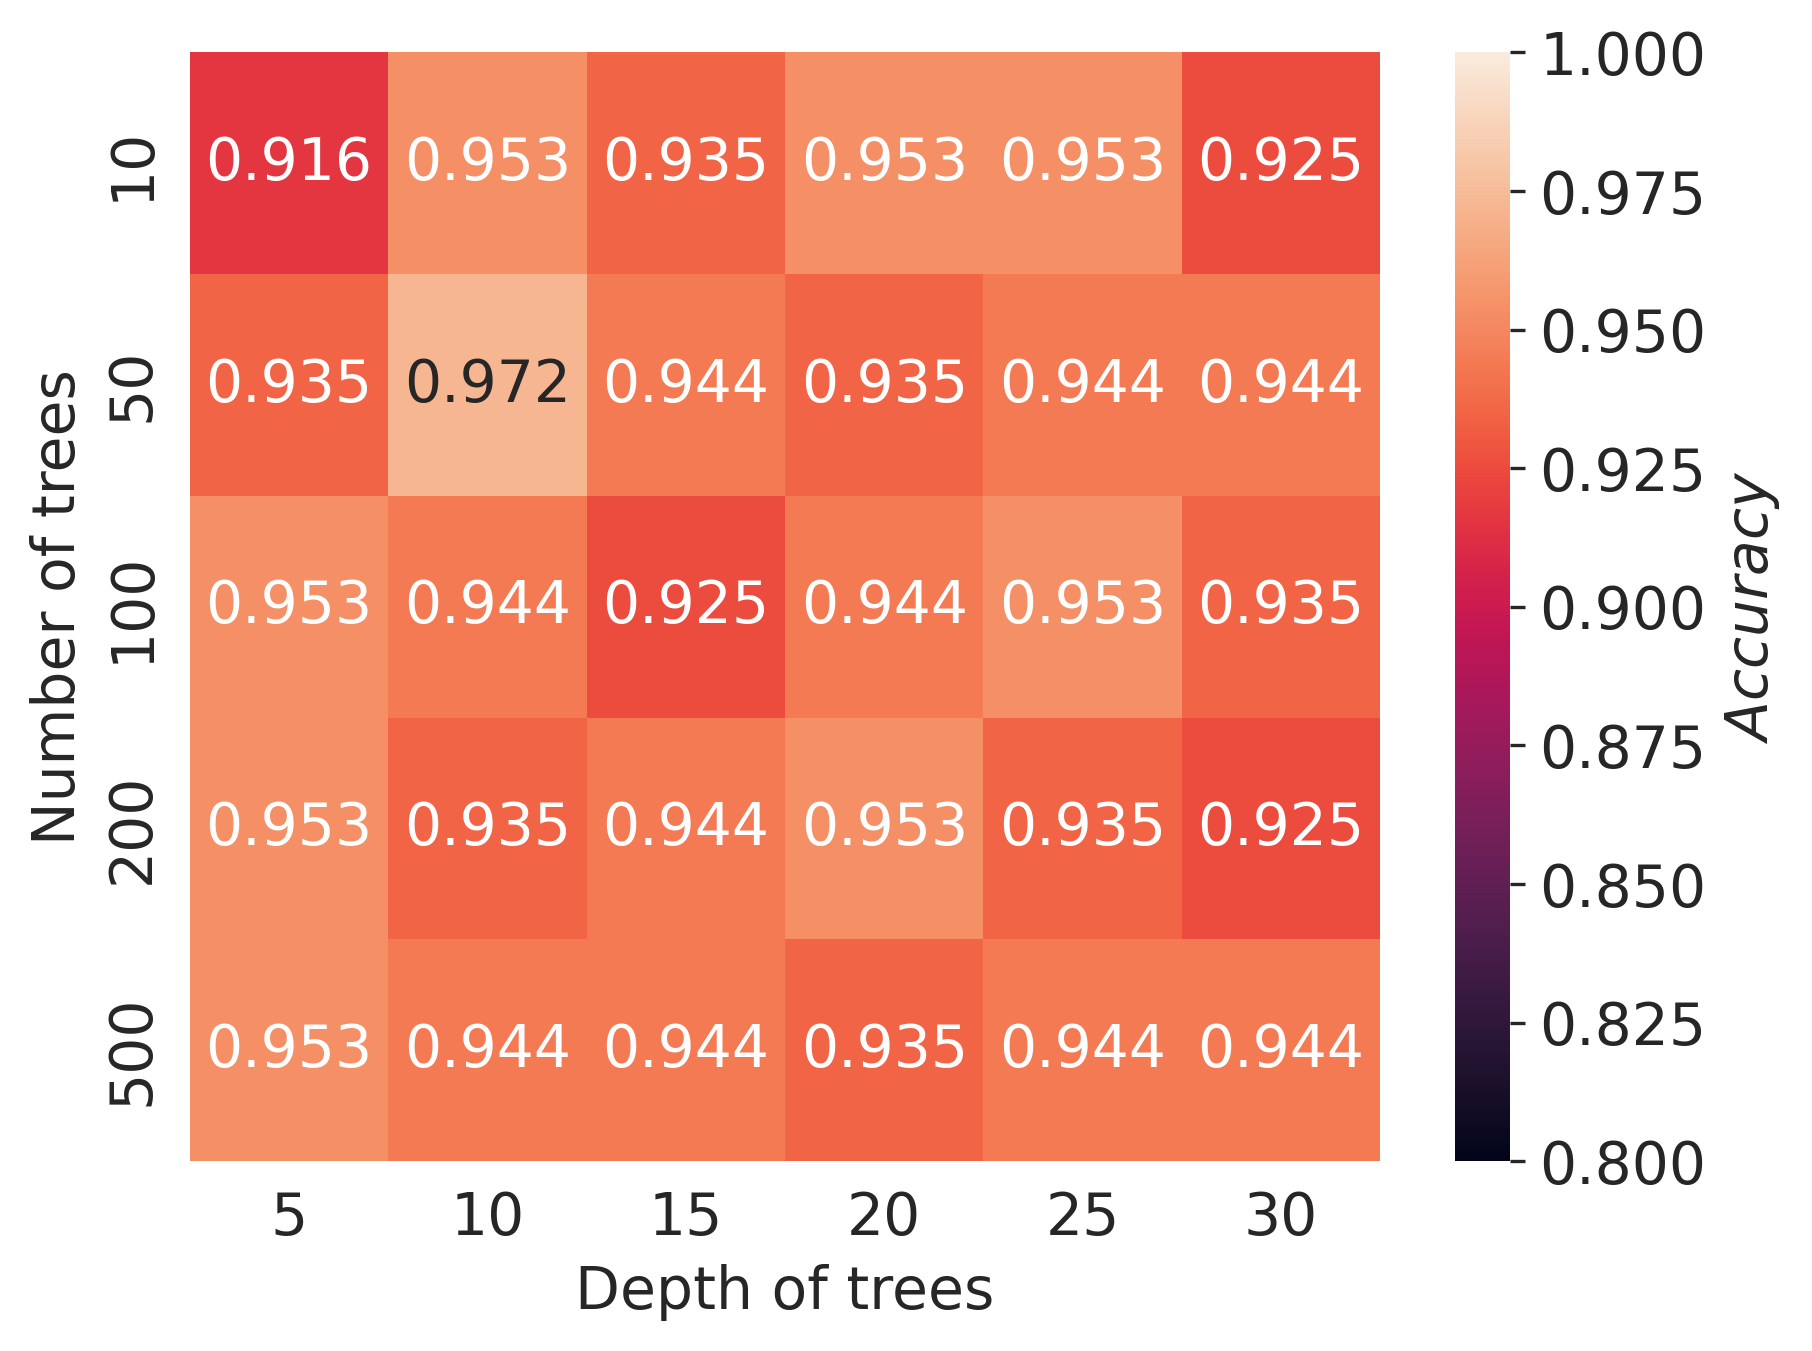
\includegraphics[width=.5\textwidth]{../figures/RF_grid_test.png}
    \caption{16-wind compass rose used to describe wind directions. Labels are defined as N (North), S (South), W (West) and E (East).}
    \label{fig:compass}
\end{figure}
\begin{figure}
    \centering
    
\includegraphics[width=.5\textwidth]{../figures/Brosen_windrose.png}
    \caption{16-wind compass rose used to describe wind directions. Labels are defined as N (North), S (South), W (West) and E (East).}
    \label{fig:compass}
\end{figure}
\begin{table}[H]
    \begin{small}
        \caption{}
        \label{tab:compass}
        \begin{center}
            \begin{tabular}{|c|c|c|c|c|c|c|c|c|c|c|c|c|c|c|c|}
                \hline
                N & NNE & NE & ENE & E & ESE & SE & SSE & S & SSW & SW & WSW & W  & WNW & NW & NNW \\
                \hline
                0 & 1   & 2  & 3   & 4 & 5   & 6  & 7   & 8 & 9   & 10 & 11  & 12 & 13  & 14 & 15  \\
                \hline
            \end{tabular}
        \end{center}
    \end{small}
\end{table}

\newpage
\appendix
\section{Dataset}
\label{app:dataset}
\begin{table}[H]
    \begin{small}
        \caption{Description of dataset features to predict the last feature "RainTomorrow" if it is going to rain tomorrow or not }
        \label{tab:features}
        \begin{center}
            \begin{tabular}{|l|l|l|}
                \hline
                \textbf{Feature} & \textbf{desctiption}                                 & \textbf{Unit}           \\
                \hline
                \hline
                Location         & Common name of the weather station                   & name                    \\
                \hline
                MinTemp          & Minimum temperature                                  & degrees Celcius         \\
                \hline
                MaxTemp          & Maximum temperature                                  & degrees Celcius         \\
                \hline
                Rainfall         & Amount of rainfall recorded in the day               & mm                      \\
                \hline
                Evaporation      & The "Class A" pan evaporation in the 24 hours        & mm                      \\
                \hline
                Sunshine         & Number of hours with bright sunshine in the day      & hours                   \\
                \hline
                WindGustDir      & direction of the strongest wind gust in the 24 hours & 16-wind compass rose    \\
                \hline
                WindGustSpeed    & Speed of the strongest wind gust in the 24 hours     & km/h                    \\
                \hline
                WindDir9am       & wind direction at 9am                                & 16-wind compass rose    \\
                \hline
                WindDir3pm       & wind direction at 3pm                                & 16-wind compass rose    \\
                \hline
                WindSpeed9am     & Wind speed at 9am                                    & km/h                    \\
                \hline
                WindSpeed3pm     & Wind speed at 3pm                                    & km/h                    \\
                \hline
                Humidity9am      & Relative humidity at 9am                             & percent                 \\
                \hline
                Humidity3pm      & Relative humidity at 3pm                             & percent                 \\
                \hline
                Pressure9am      & Pressure reduced to mean sea level at 9am            & hPa                     \\
                \hline
                Pressure3pm      & Pressure reduced to mean sea level at 3pm            & hPa                     \\
                \hline
                Cloud9am         & Fraction of sky covered by clouds at 9am             & oktas (units of eights) \\
                \hline
                Cloud3pm         & Fraction of sky covered by clouds at 3pm             & oktas (units of eights) \\
                \hline
                Temp9am          & Temperature at 9am                                   & degrees Celcius         \\
                \hline
                Temp3pm          & Temperature at 3pm                                   & degrees Celcius         \\
                \hline
                RainToday        & Rain exceeding 1mm over 24 hours today               & Yes or No               \\
                \hline
                RainTomorrow     & Rain exceeding 1mm over 24 hours tomorrow            & Yes or No               \\
                \hline
            \end{tabular}
        \end{center}
    \end{small}
\end{table}

\end{document}